% Options for packages loaded elsewhere
\PassOptionsToPackage{unicode}{hyperref}
\PassOptionsToPackage{hyphens}{url}
%
\documentclass[
]{article}
\usepackage{amsmath,amssymb}
\usepackage{lmodern}
\usepackage{iftex}
\ifPDFTeX
  \usepackage[T1]{fontenc}
  \usepackage[utf8]{inputenc}
  \usepackage{textcomp} % provide euro and other symbols
\else % if luatex or xetex
  \usepackage{unicode-math}
  \defaultfontfeatures{Scale=MatchLowercase}
  \defaultfontfeatures[\rmfamily]{Ligatures=TeX,Scale=1}
\fi
% Use upquote if available, for straight quotes in verbatim environments
\IfFileExists{upquote.sty}{\usepackage{upquote}}{}
\IfFileExists{microtype.sty}{% use microtype if available
  \usepackage[]{microtype}
  \UseMicrotypeSet[protrusion]{basicmath} % disable protrusion for tt fonts
}{}
\makeatletter
\@ifundefined{KOMAClassName}{% if non-KOMA class
  \IfFileExists{parskip.sty}{%
    \usepackage{parskip}
  }{% else
    \setlength{\parindent}{0pt}
    \setlength{\parskip}{6pt plus 2pt minus 1pt}}
}{% if KOMA class
  \KOMAoptions{parskip=half}}
\makeatother
\usepackage{xcolor}
\usepackage[margin=1in]{geometry}
\usepackage{graphicx}
\makeatletter
\def\maxwidth{\ifdim\Gin@nat@width>\linewidth\linewidth\else\Gin@nat@width\fi}
\def\maxheight{\ifdim\Gin@nat@height>\textheight\textheight\else\Gin@nat@height\fi}
\makeatother
% Scale images if necessary, so that they will not overflow the page
% margins by default, and it is still possible to overwrite the defaults
% using explicit options in \includegraphics[width, height, ...]{}
\setkeys{Gin}{width=\maxwidth,height=\maxheight,keepaspectratio}
% Set default figure placement to htbp
\makeatletter
\def\fps@figure{htbp}
\makeatother
\setlength{\emergencystretch}{3em} % prevent overfull lines
\providecommand{\tightlist}{%
  \setlength{\itemsep}{0pt}\setlength{\parskip}{0pt}}
\setcounter{secnumdepth}{-\maxdimen} % remove section numbering
\usepackage{booktabs}
\usepackage{longtable}
\usepackage{array}
\usepackage{multirow}
\usepackage{wrapfig}
\usepackage{float}
\usepackage{colortbl}
\usepackage{pdflscape}
\usepackage{tabu}
\usepackage{threeparttable}
\usepackage{threeparttablex}
\usepackage[normalem]{ulem}
\usepackage{makecell}
\usepackage{xcolor}
\ifLuaTeX
  \usepackage{selnolig}  % disable illegal ligatures
\fi
\IfFileExists{bookmark.sty}{\usepackage{bookmark}}{\usepackage{hyperref}}
\IfFileExists{xurl.sty}{\usepackage{xurl}}{} % add URL line breaks if available
\urlstyle{same} % disable monospaced font for URLs
\hypersetup{
  pdftitle={Three (Groups of) Blind Mice},
  pdfauthor={Alyssa Allsop and Amira Burns},
  hidelinks,
  pdfcreator={LaTeX via pandoc}}

\title{Three (Groups of) Blind Mice}
\usepackage{etoolbox}
\makeatletter
\providecommand{\subtitle}[1]{% add subtitle to \maketitle
  \apptocmd{\@title}{\par {\large #1 \par}}{}{}
}
\makeatother
\subtitle{Familial Clusters of Cataract Development in Irradiated Mice}
\author{Alyssa Allsop and Amira Burns}
\date{2022-06-20}

\begin{document}
\maketitle

\hypertarget{abstract}{%
\subsection{Abstract}\label{abstract}}

\hypertarget{introduction}{%
\subsection{Introduction}\label{introduction}}

Little is known about the effects of high atomic number and energy (HZE)
radiation, a main component of space radiation to which exposure is
unavoidable beyond Earth's magnetic field. In contrast, extensive
research shows exposure to high doses of gamma radiation leads to acute
radiation sickness. Effects include damage to the blood forming system,
GI system, immune system, increased risk for cancer, cardiovascular
disease, neurodegenerative disease, death, and cataracts.. The serious
health implications from HZE radiation for astronauts who leave Earth's
magnetic field warrant further study. Adverse effects from radiation may
also be attributable to other factors, including genetics; several
different cancers have been observed to cluster in mice families
(Chernyavskiy, et. al., 2017). Accounting for potential family
clustering allows for thorough examination of the primary research
questions. Is there a genetic susceptibility to cataracts caused by
radiation? Accounting for potential genetic susceptibility, is there a
difference in cataract presentation between HZE radiation and gamma
radiation? The full dataset includes 1820 unique mice from 48 unique
families, with equal random assignments by family to each of three
treatment groups. Mice are bred over several generations to create a
genetically heterogeneous sample, the better to represent the diverse
biology of the human population. The treatments are HZE irradiation,
gamma irradiation, and non-irradiated control. The HZE group is
irradiated with either silicon or iron nuclei HZE ions, which are
considered as a single treatment group. The second group is subjected to
137 Cs gamma irradiation. Mice in both irradiated groups are exposed to
radiation at 7-12 weeks of age. The third group is unirradiated control.
All mice are monitored until 800 days of age --effectively a survival
study. Mice are checked weekly for symptoms of cataracts, cataract risk
factors, and other symptoms of radiation exposure such as tumors and
carcinomas. Resources do not allow for weekly measurement of every
mouse; previous measurements are carried forward if a mouse is not
assessed on a particular week. This analysis uses a simplified version
of the data set - a snapshot of the 1169 mice that are alive at 552
days. This cutoff is chosen because it is the median survival time for
the group with the shortest median survival. There are 47 unique
families with n = 396 in the HZE group, n = 277 in the gamma radiation
group, and n = 496 in the unirradiated control group. There are up to
two generations of mice pups from each family in the dataset, but
generation is not distinguished in the simplified data. Family size
ranges from n = 11 to n = 48, with median family size of 24.

\begin{wraptable}{r}{0pt}

\caption{\label{tab:scoregrps}Counts of Score by Treatment}
\centering
\fontsize{12}{14}\selectfont
\begin{tabular}[t]{l|r|r|r|r|r}
\hline
\multicolumn{1}{c|}{ } & \multicolumn{4}{c|}{Cataract Score} & \multicolumn{1}{c}{ } \\
\cline{2-5}
Treatment & 1 & 2 & 3 & 4 & Total\\
\hline
Unirradiated & 438 & 45 & 11 & 2 & 496\\
\hline
Gamma & 214 & 53 & 6 & 4 & 277\\
\hline
HZE & 281 & 107 & 6 & 2 & 396\\
\hline
\end{tabular}
\end{wraptable}

The response is Merriam-Focht cataract score (Merriam \& Focht, 1957),
an ordinal categorical variable corresponding to radiation-associated
ocular changes in the eye. A score of 0 is associated with a completely
clear lens, while a score of 5 is associated with a completely occluded
lens. This dataset contains cataract score levels = {[}1, 2, 3, 4{]}. A
score \(\ge\) 2 indicates presence of cataracts, and the small sample
sizes for score \(>\) 2 across all treatment groups raise concerns about
making inference on an ordinal analysis; consequently, the response is
converted to binary \emph{Cataracts} with score = 1 converted to 0, and
score \(\ge\) 2 converted to 1. The main experimental factor is
\emph{Treatment}, a categorical variable with three levels = {[}HZE
radiation, gamma radiation, non-irradiated control{]}. A single random
effect, genetic \emph{Family}, is a categorical factor with 47 levels.
Both Treatment and Family are central to the experimental design and
will serve as the basis for all models considered. Additional covariates
under consideration are:\\
+ Sex: categorical with two levels = {[}Male, Female{]}.\\
+ Weight: numeric, in grams; range = {[}16.11, 59.85{]}.\\
+ Coat color: categorical with six levels = {[}albino, black, creme
brown, grey, light brown, light grey{]}.\\
+ Body condition score (BCS): ordered categorical with 5 levels,
representing a range from emaciated to obese. Levels = {[}BC1, BC2, BC3,
BC4, BC5{]}.\\
+ Age: numeric, in days; range = {[}552, 816{]}.\\
+ Three categorical variables indicating presence of other cancers:
Harderian Tumor: categorical with three levels = {[}bilateral,
unilateral, none{]}. Myeloid Leukemia: binary categorical with two
levels = {[}0, 1{]}. PreT Lymphoma: binary categorical with two levels =
{[}0, 1{]}.

The experimental design prescribed the inclusion of Treatment and Family
in a final model.

\hypertarget{summary-statistics}{%
\subsection{Summary Statistics}\label{summary-statistics}}

Exploratory data analysis consisted of investigating the response in
terms of Treatment and Family and any potential associations between the
response and covariates. In addition, possible interactions and
correlations between covariates and the primary predictors in terms of
the response were of interest.

\begin{table}[!h]

\caption{\label{tab:table}Mice Counts and Percentages by Sex, Treatment Group, Cataracts}
\centering
\begin{tabular}[t]{l|l|r|r|r|r|r|r}
\hline
\multicolumn{2}{c|}{ } & \multicolumn{2}{c|}{Female} & \multicolumn{2}{c|}{Male} & \multicolumn{2}{c}{\$\textbackslash{}sum\$} \\
\cline{3-4} \cline{5-6} \cline{7-8}
Treatment & Cataracts & n & prop & n & prop & n & prop\\
\hline
\multicolumn{8}{l}{\textbf{Control}}\\
\hline
\hspace{1em} & No & 238 & 0.92 & 200 & 0.84 & 438 & 0.88\\
\hline
\hspace{1em} & Yes & 20 & 0.08 & 38 & 0.16 & 58 & 0.12\\
\hline
\hspace{1em} & \$\textbackslash{}sum\$ & 258 &  & 238 &  & 496 & \\
\hline
\multicolumn{8}{l}{\textbf{Gamma}}\\
\hline
\hspace{1em} & No & 131 & 0.90 & 83 & 0.63 & 214 & 0.77\\
\hline
\hspace{1em} & Yes & 14 & 0.10 & 49 & 0.37 & 63 & 0.23\\
\hline
\hspace{1em} & \$\textbackslash{}sum\$ & 145 &  & 132 &  & 277 & \\
\hline
\multicolumn{8}{l}{\textbf{HZE}}\\
\hline
\hspace{1em} & No & 181 & 0.88 & 100 & 0.52 & 281 & 0.71\\
\hline
\hspace{1em} & Yes & 24 & 0.12 & 91 & 0.48 & 115 & 0.29\\
\hline
\hspace{1em} & \$\textbackslash{}sum\$ & 205 &  & 191 &  & 396 & \\
\hline
\multicolumn{8}{l}{\textbf{\$\textbackslash{}sum\$}}\\
\hline
\hspace{1em} & \$\textbackslash{}sum\$ & 608 &  & 561 &  & 1169 & \\
\hline
\end{tabular}
\end{table}

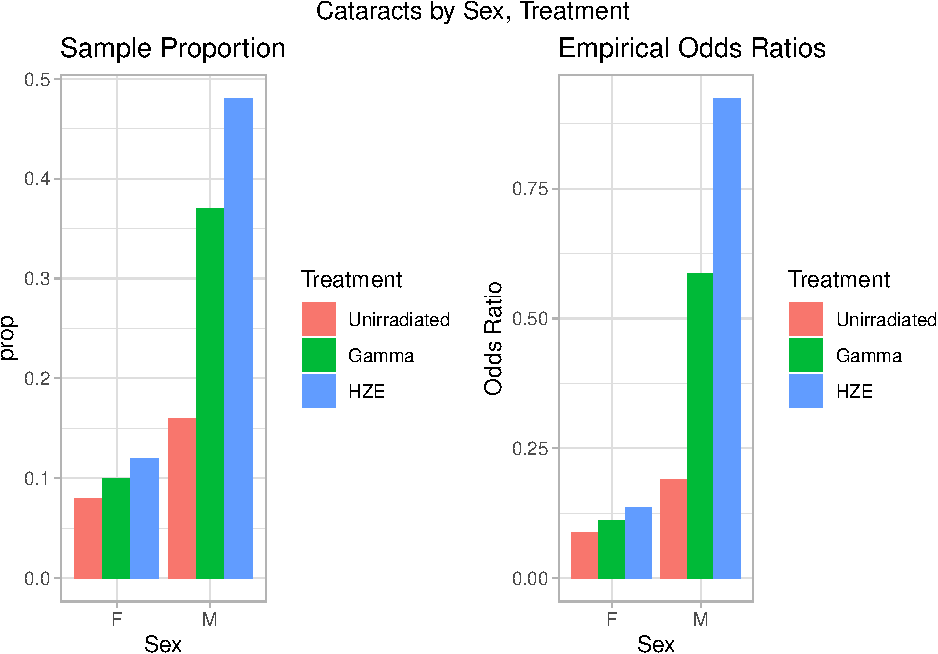
\includegraphics{final_report_files/figure-latex/barplot-1.pdf}

\hypertarget{statistical-methods}{%
\subsection{Statistical Methods}\label{statistical-methods}}

\hypertarget{frequentist-approach}{%
\subsubsection{Frequentist Approach}\label{frequentist-approach}}

\begin{verbatim}
## Generalized linear mixed model fit by maximum likelihood (Laplace
##   Approximation) [glmerMod]
##  Family: binomial  ( logit )
## Formula: Cataracts ~ Treatment * Sex + (1 | Family)
##    Data: cats
## 
##      AIC      BIC   logLik deviance df.resid 
##   1018.0   1053.4   -502.0   1004.0     1162 
## 
## Scaled residuals: 
##     Min      1Q  Median      3Q     Max 
## -1.9388 -0.4201 -0.3050 -0.2193  4.7063 
## 
## Random effects:
##  Groups Name        Variance Std.Dev.
##  Family (Intercept) 0.3949   0.6284  
## Number of obs: 1169, groups:  Family, 47
## 
## Fixed effects:
##                     Estimate Std. Error z value Pr(>|z|)    
## (Intercept)          -2.6973     0.2608 -10.343  < 2e-16 ***
## TreatmentGamma        0.2137     0.3705   0.577  0.56409    
## TreatmentHZE          0.5007     0.3239   1.546  0.12214    
## SexM                  0.8875     0.2981   2.977  0.00291 ** 
## TreatmentGamma:SexM   0.9748     0.4548   2.144  0.03207 *  
## TreatmentHZE:SexM     1.2068     0.4020   3.002  0.00269 ** 
## ---
## Signif. codes:  0 '***' 0.001 '**' 0.01 '*' 0.05 '.' 0.1 ' ' 1
## 
## Correlation of Fixed Effects:
##             (Intr) TrtmnG TrtHZE SexM   TrG:SM
## TreatmntGmm -0.571                            
## TreatmntHZE -0.666  0.464                     
## SexM        -0.730  0.501  0.578              
## TrtmntGm:SM  0.455 -0.815 -0.375 -0.648       
## TrtmnHZE:SM  0.513 -0.373 -0.800 -0.733  0.487
\end{verbatim}

\hypertarget{bayesian-approach}{%
\subsubsection{Bayesian Approach}\label{bayesian-approach}}

We fit a complementary Bayesian model to examine the distribution of the
estimates from our final model, as well as test its robustness to
alternative approaches. The Bayes model is parameterized as:

\[
\begin{aligned}
Y_{ij} \sim &Bernoulli(p)\\
log(\frac{p}{1-p}) = &\ \beta_0*Control_i*F_i\ +\beta_1*Gamma_i*F_i\ + \beta_2*HZE_i*F_i\ + \\ &\beta_3*Control_i*M_i\ +\beta_4*Gamma*M\ + \beta_5*HZE*M\ + \\
&v_{j} + \epsilon_{ij}\\
&i = 1, ..., 1169\ \mbox{ mice} \\
&j = 1,...,47\ \ \mbox{ families, and} \\
v_j \sim\ &N(0, \tau)
\end{aligned}
\]

With non-informative parameters:\\
\[
\begin{aligned}
\beta_0 &\sim N(0, 0.001)\\
\beta_1 &\sim N(0, 0.001)\\
\beta_2 &\sim N(0, 0.001)\\
\beta_3 &\sim N(0, 0.001)\\
\beta_4 &\sim N(0, 0.001)\\
\beta_5 &\sim N(0, 0.001)\\
v_i &\sim N(0, \sigma^2)\\
\tau &\sim Gamma(0.001, 0.001) \mbox{ where}\ \sigma^2 = 1/\tau\\
\end{aligned}
\]

The model was run through a Gibbs sampler Markov Chain Monte Carlo
(MCMC) algorithm to approximate the posterior distribution of all fixed
effects estimates and the variance of the random effect. 3 chains of
60000 total iterations with a 10000-iteration burn-in period; starting
values were obtained from the estimates generated by the Frequentist
model, with noise added to avoid false convergence.

\begin{verbatim}
## Compiling model graph
##    Resolving undeclared variables
##    Allocating nodes
## Graph information:
##    Observed stochastic nodes: 1169
##    Unobserved stochastic nodes: 54
##    Total graph size: 6473
## 
## Initializing model
\end{verbatim}

\begin{wraptable}{l}{0pt}

\caption{\label{tab:bayes_tab}Final Model Parameter Estimates (probabilities)}
\centering
\begin{tabular}[t]{l|r|r|r|r|r|r|r}
\hline
  & GLMM Est & MCMC Mean & MCMC Median & MCMC Mode & MCMC SD & HPD Lower & HPD Upper\\
\hline
\$\textbackslash{}beta\_0\$ & 0.063 & 0.063 & 0.062 & 0.057 & 0.016 & 0.034 & 0.094\\
\hline
\$\textbackslash{}beta\_1\$ & 0.553 & 0.549 & 0.551 & 0.550 & 0.090 & 0.371 & 0.720\\
\hline
\$\textbackslash{}beta\_2\$ & 0.623 & 0.621 & 0.624 & 0.634 & 0.076 & 0.469 & 0.764\\
\hline
\$\textbackslash{}beta\_3\$ & 0.708 & 0.708 & 0.710 & 0.714 & 0.062 & 0.589 & 0.828\\
\hline
\$\textbackslash{}beta\_4\$ & 0.726 & 0.721 & 0.729 & 0.723 & 0.090 & 0.544 & 0.883\\
\hline
\$\textbackslash{}beta\_5\$ & 0.770 & 0.763 & 0.771 & 0.776 & 0.072 & 0.618 & 0.892\\
\hline
\$\textbackslash{}sigma\textasciicircum{}2\$ & 0.597 & 0.609 & 0.604 & 0.585 & 0.041 & 0.539 & 0.694\\
\hline
\end{tabular}
\end{wraptable}

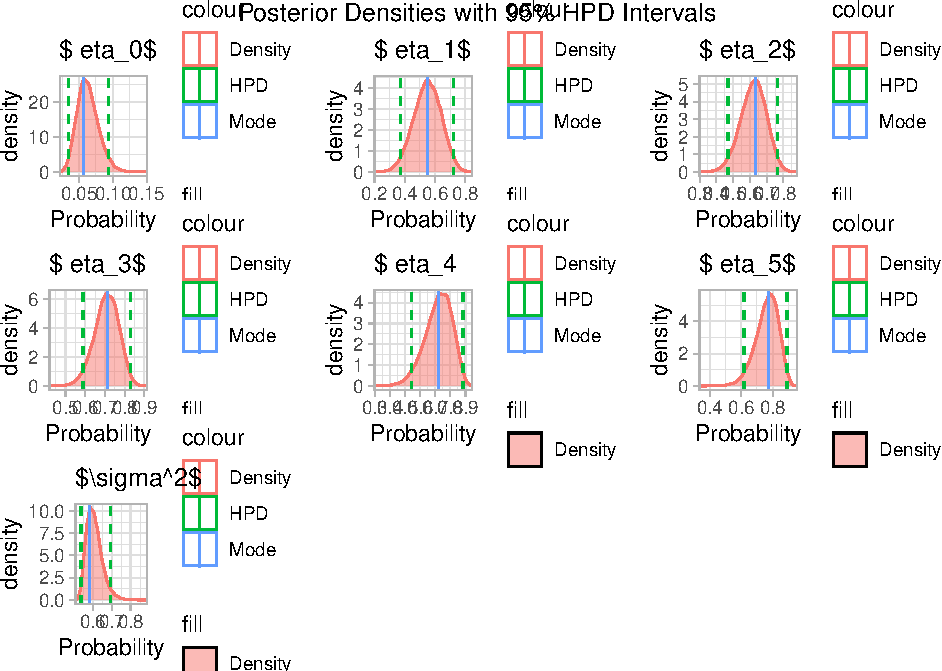
\includegraphics{final_report_files/figure-latex/postdens-1.pdf}

\hypertarget{limitations-and-alternatives}{%
\subsection{Limitations and
Alternatives}\label{limitations-and-alternatives}}

Presence of competing risks in the experimental design obscure the
presence of family clusters of cataracts. It is reasonable to assume
that individuals in the irradiated Treatment groups were more likely to
die due to more acute effects of irradiation before developing
cataracts, compared to individuals in the control group. Simplifying the
dataset by instituting a cutoff age attempts to address this limitation,
but the issue persists even after excluding individuals deceased before
Age = 552.

\hypertarget{results-and-conclusions}{%
\subsection{Results and Conclusions}\label{results-and-conclusions}}

The final probability for developing cataracts can be written as:\\
\[
p_i = 0.063 + 0.55*Gamma_i + 0.623*HZE_i + 0.708*Male_i + 0.726*Gamma_i*Male_i + 0.770*HZE_i*Male_i
\]

\begin{verbatim}
## Sex = F:
##  Treatment      prob     SE  df asymp.LCL asymp.UCL null z.ratio p.value
##  Unirradiated 0.0631 0.0154 Inf    0.0389     0.101  0.5 -10.343  <.0001
##  Gamma        0.0770 0.0219 Inf    0.0436     0.132  0.5  -8.062  <.0001
##  HZE          0.1001 0.0221 Inf    0.0643     0.153  0.5  -8.942  <.0001
## 
## Sex = M:
##  Treatment      prob     SE  df asymp.LCL asymp.UCL null z.ratio p.value
##  Unirradiated 0.1407 0.0252 Inf    0.0982     0.198  0.5  -8.697  <.0001
##  Gamma        0.3495 0.0485 Inf    0.2613     0.449  0.5  -2.913  0.0036
##  HZE          0.4744 0.0448 Inf    0.3882     0.562  0.5  -0.569  0.5693
## 
## Confidence level used: 0.95 
## Intervals are back-transformed from the logit scale 
## Tests are performed on the logit scale
\end{verbatim}

\begin{verbatim}
## Sex = F:
##  contrast             odds.ratio    SE  df null z.ratio p.value
##  Gamma / Unirradiated       1.24 0.459 Inf    1   0.577  0.8325
##  HZE / Unirradiated         1.65 0.534 Inf    1   1.546  0.2695
##  HZE / Gamma                1.33 0.482 Inf    1   0.793  0.7071
## 
## Sex = M:
##  contrast             odds.ratio    SE  df null z.ratio p.value
##  Gamma / Unirradiated       3.28 0.865 Inf    1   4.509  <.0001
##  HZE / Unirradiated         5.51 1.331 Inf    1   7.076  <.0001
##  HZE / Gamma                1.68 0.412 Inf    1   2.115  0.0868
## 
## P value adjustment: tukey method for comparing a family of 3 estimates 
## Tests are performed on the log odds ratio scale
\end{verbatim}

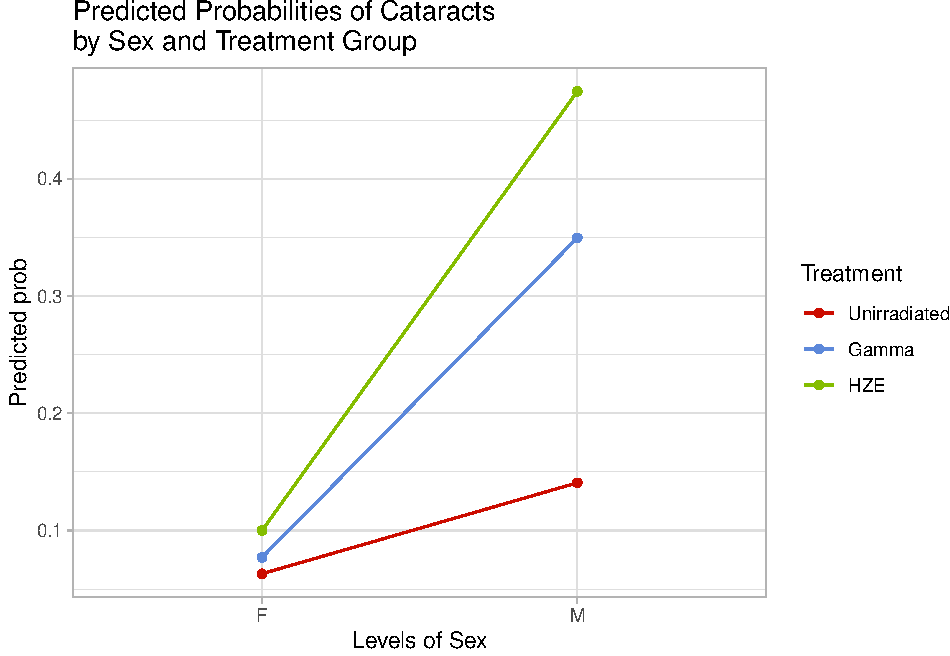
\includegraphics{final_report_files/figure-latex/contr-1.pdf}

Assessing odds ratios for cataracts between groups:

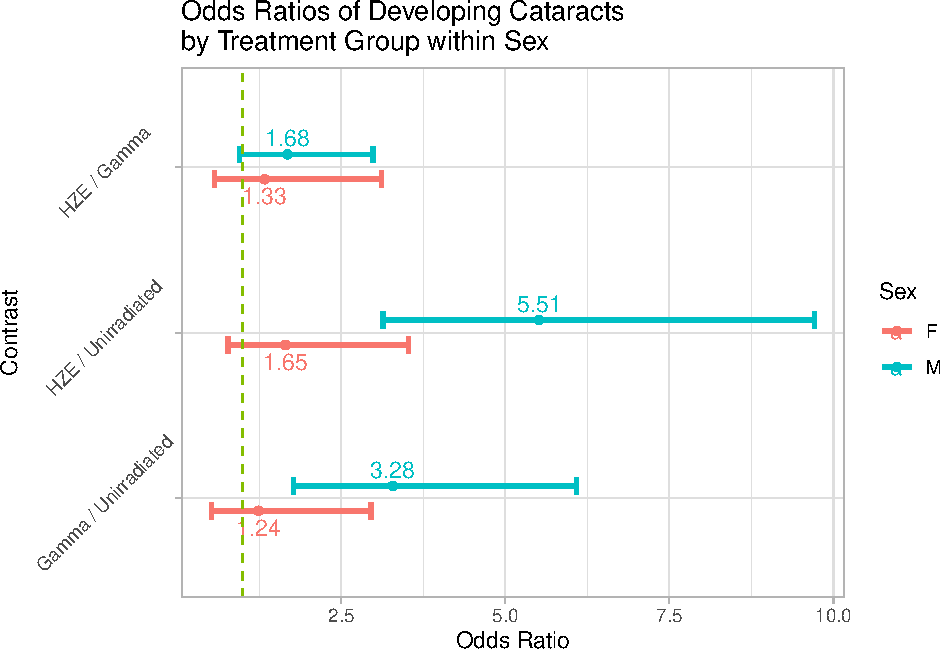
\includegraphics{final_report_files/figure-latex/oddsr-1.pdf}

\begin{verbatim}
## Treatment = Unirradiated:
##  contrast odds.ratio    SE  df null z.ratio p.value
##  M / F          2.43 0.724 Inf    1   2.977  0.0029
## 
## Treatment = Gamma:
##  contrast odds.ratio    SE  df null z.ratio p.value
##  M / F          6.44 2.231 Inf    1   5.374  <.0001
## 
## Treatment = HZE:
##  contrast odds.ratio    SE  df null z.ratio p.value
##  M / F          8.12 2.220 Inf    1   7.658  <.0001
## 
## Tests are performed on the log odds ratio scale
\end{verbatim}

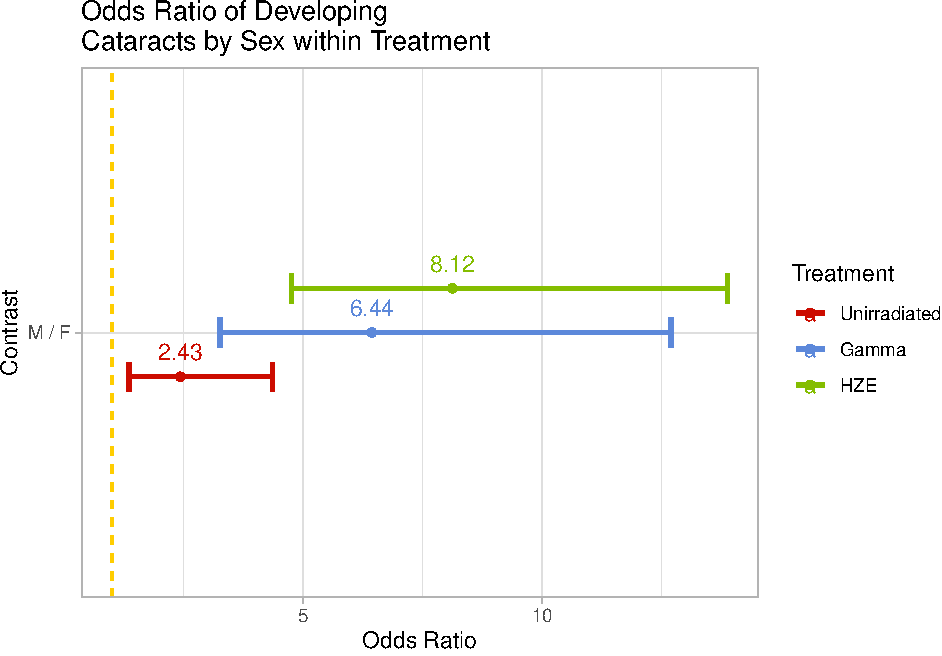
\includegraphics{final_report_files/figure-latex/oddsr2-1.pdf}

Assessing relative risk for cataracts between groups:\\
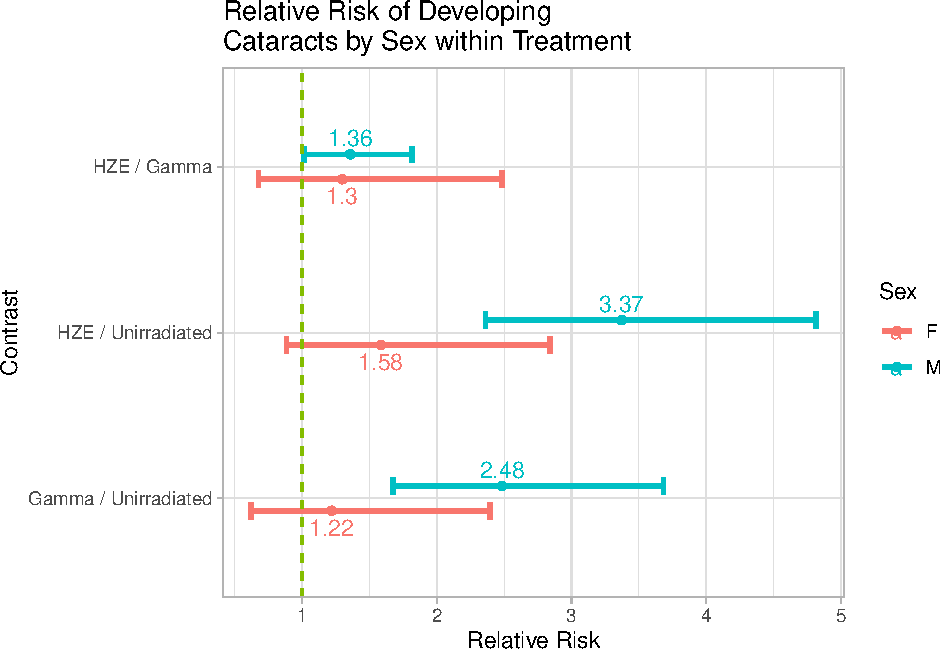
\includegraphics{final_report_files/figure-latex/RR-1.pdf}

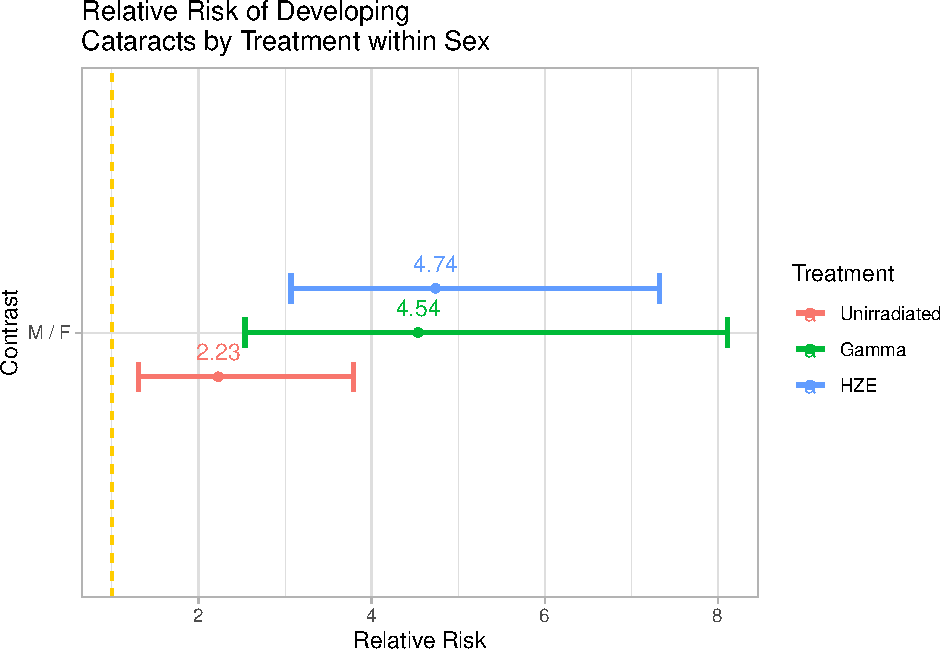
\includegraphics{final_report_files/figure-latex/RR1-1.pdf}

Visualizing random effect by family:\\
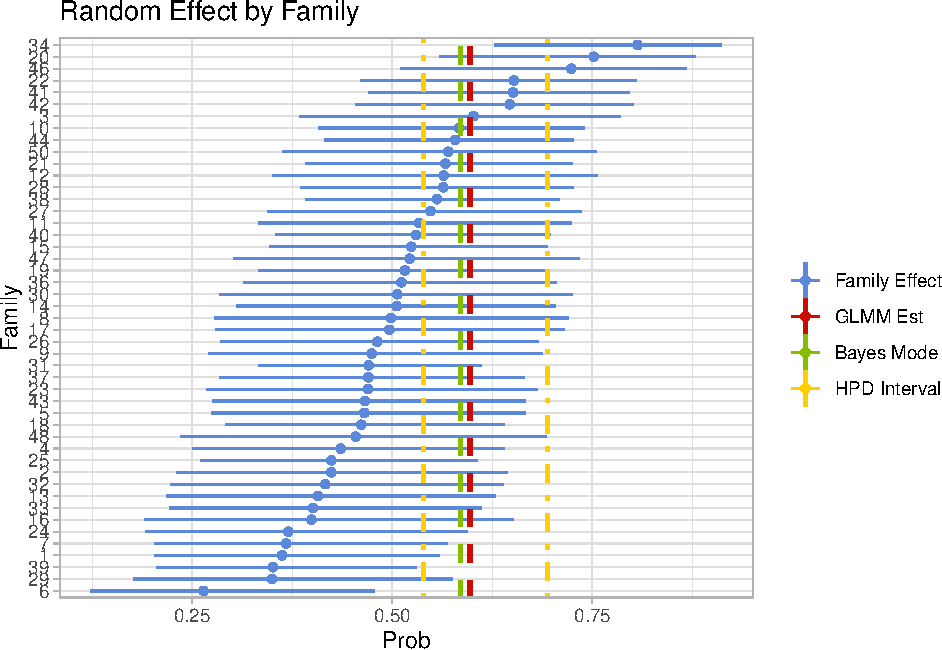
\includegraphics{final_report_files/figure-latex/re_plot-1.pdf}

\hypertarget{authors-statements}{%
\subsection{Authors' Statements}\label{authors-statements}}

Both authors contributed to statistical analysis and writing for this
report. Both authors read and approved the final report. Both authors
contributed equally to introduction, exploratory data analysis, summary
statistics, and results. Alyssa Allsop served as the primary
statistician on fitting Frequentist models; Amira Burns served as the
primary statistician on fitting the Bayesian model.

\hypertarget{references}{%
\subsection{References}\label{references}}

Agresti, A (2013). \emph{Categorical Data Analysis} (Third Edition).
John Wiley \& Sons.

Chernyavskiy, P., Edmondson, E. F., Weil, M. M., \& Little, M. P.
(2017). \emph{High-energy particle beam and gamma radiation exposure,
familial relatedness and cancer in mice.} British journal of cancer,
117(1), 41--50. \url{https://doi.org/10.1038/bjc.2017.141}

Gelman, A., Carlin, J., Stern, H., Dunson, D., Vehtari, A., Rubin, D.
(2014). \emph{Bayesian Data Analysis} (Third Edition). CRC Press.

Roback, P., Legler, J. (2021). \emph{Beyond Multiple Linear Regression.
Applied Generalized Linear Models and Multilevel Models in R} (Second
Edition). CRC Press. Online version:
\url{https://bookdown.org/roback/bookdown-BeyondMLR/}

DiMaggio, C., Albert, J., Spiegelhalter, D., Best, N., Gelman, A.,
Carstensen, B., Guerrin, L., Jensen, S. (2015) \emph{Bayesian Analysis
for Epidemiologists III: Regression Modeling.} Center for Injury
Epidemiology and Prevention at Columbia University.
\url{http://www.columbia.edu/~cjd11/charles_dimaggio/DIRE/styled-4/styled-11/code-8/\#bayesian-regression-modeling-with-bugs-or-jags}

R Packages:\\
+ Douglas Bates, Martin Maechler, Ben Bolker, Steve Walker (2015).
Fitting Linear Mixed-Effects Models Using lme4. Journal of Statistical
Software, 67(1), 1-48. \url{doi:10.18637/jss.v067.i01}.\\
+ Martyn Plummer (2021). rjags: Bayesian Graphical Models using MCMC. R
package version 4-12. \url{https://CRAN.R-project.org/package=rjags}\\
+ Russell V. Lenth (2022). emmeans: Estimated Marginal Means, aka
Least-Squares Means. R package version 1.7.3.
\url{https://CRAN.R-project.org/package=emmeans}

\hypertarget{appendix}{%
\subsection{Appendix}\label{appendix}}

\hypertarget{additional-exploratory-data-analysis}{%
\subsubsection{Additional Exploratory Data
Analysis}\label{additional-exploratory-data-analysis}}

\hypertarget{glmm-model-selection}{%
\subsubsection{GLMM Model Selection}\label{glmm-model-selection}}

\hypertarget{glmm-model-diagnostics-necessary}{%
\subsubsection{GLMM Model Diagnostics
(necessary?)}\label{glmm-model-diagnostics-necessary}}

\hypertarget{bayes-model-diagnostics}{%
\subsubsection{Bayes Model Diagnostics}\label{bayes-model-diagnostics}}

Traceplots:
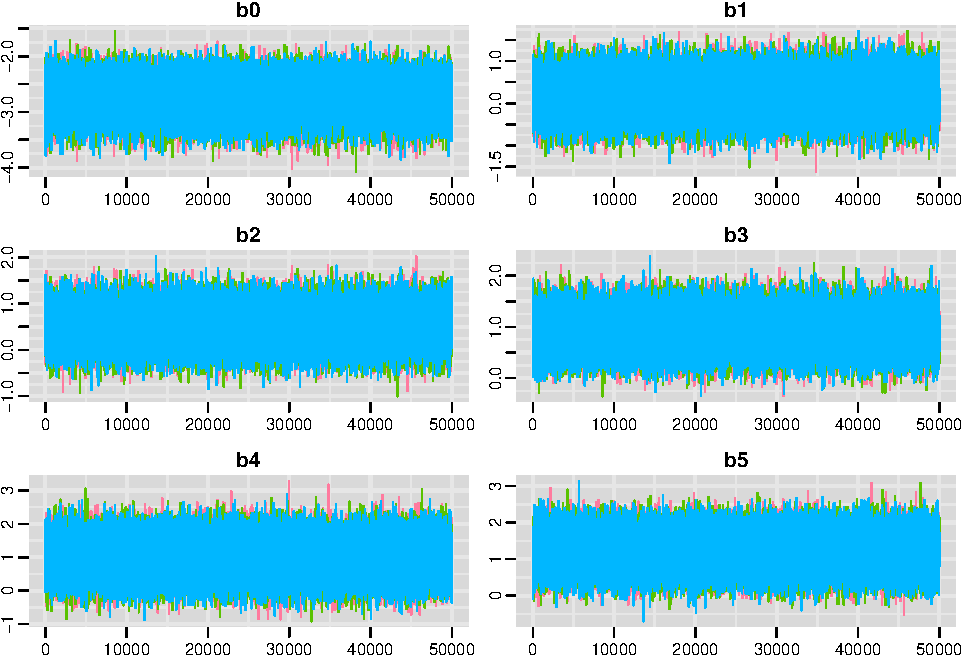
\includegraphics{final_report_files/figure-latex/trace-1.pdf}

ACF plots:\\
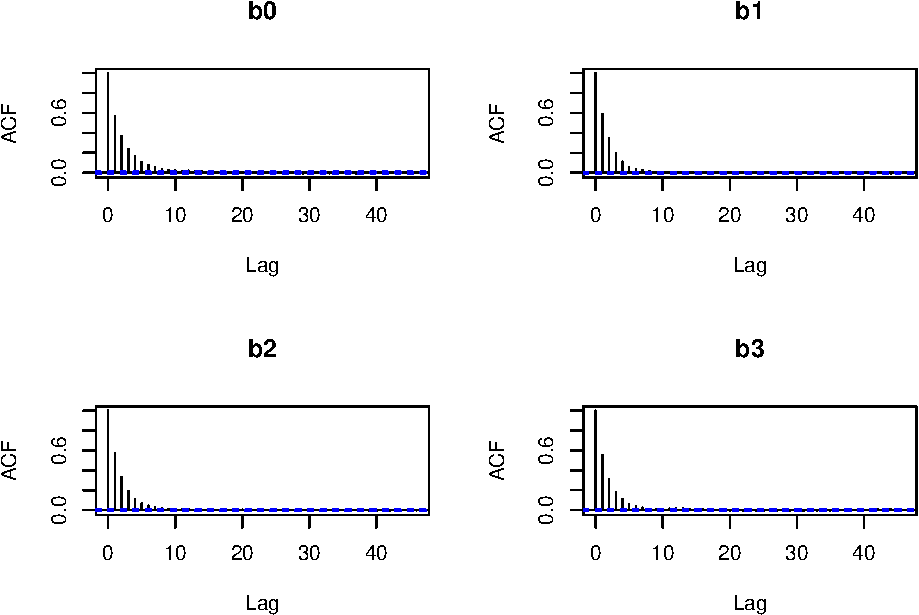
\includegraphics{final_report_files/figure-latex/acf-1.pdf}
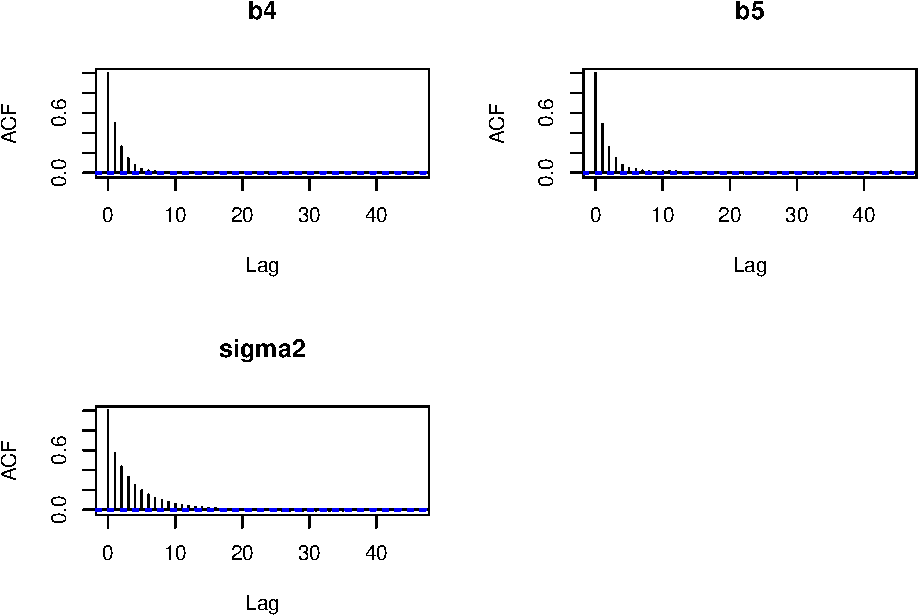
\includegraphics{final_report_files/figure-latex/acf-2.pdf} Gelman-Rubin
Diagnostics:

\begin{verbatim}
## Potential scale reduction factors:
## 
##          Point est. Upper C.I.
## b0                1          1
## b1                1          1
## b2                1          1
## b3                1          1
## b4                1          1
## b5                1          1
## deviance          1          1
## sigma2            1          1
## 
## Multivariate psrf
## 
## 1
\end{verbatim}

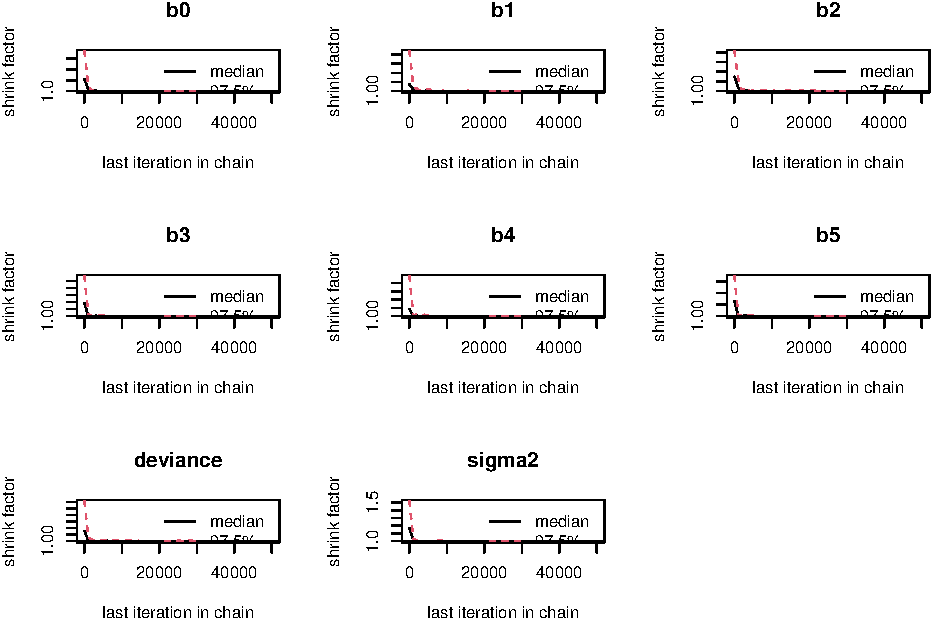
\includegraphics{final_report_files/figure-latex/grd-1.pdf}

\hypertarget{post-hoc-assessments}{%
\subsubsection{Post-Hoc Assessments}\label{post-hoc-assessments}}

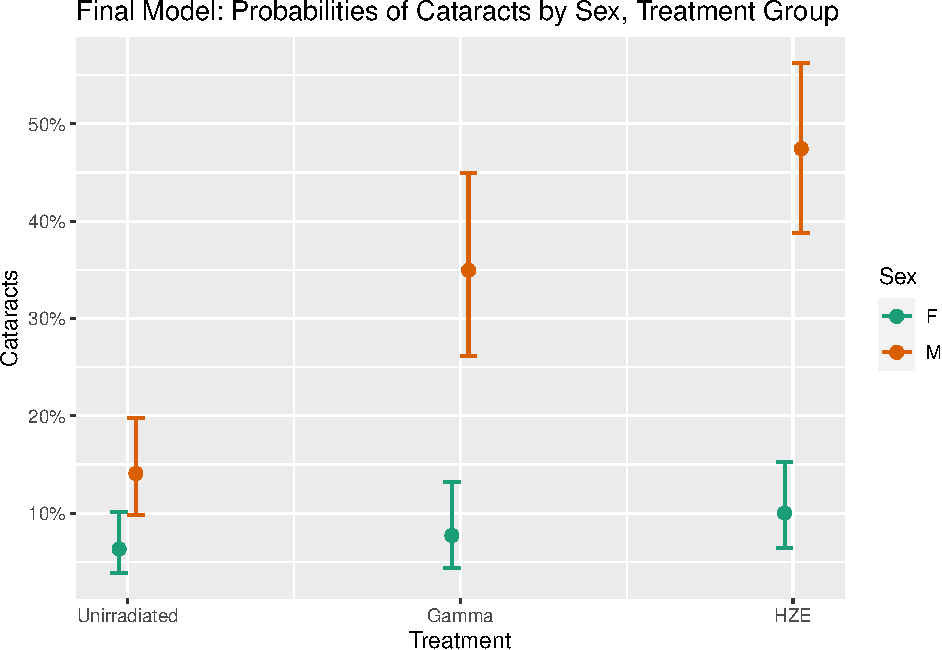
\includegraphics{final_report_files/figure-latex/glmm_ors-1.pdf}

~

Final Model: Odds Ratios of Cataracts by Sex, Treatment Group

Predictors

Odds Ratios

CI

p

Control(Female)

0.07

0.04~--~0.11

\textless0.001

Gamma(Female)

1.24

0.60~--~2.56

0.564

HZE(Female)

1.65

0.87~--~3.11

0.122

Control(Male)

2.43

1.35~--~4.36

0.003

Gamma(Male)

2.65

1.09~--~6.46

0.032

HZE(Male)

3.34

1.52~--~7.35

0.003

Random Effects

σ2

3.29

τ00 Family

0.39

ICC

0.11

N Family

47

Observations

1169

Marginal R2 / Conditional R2

0.194 / 0.281

\hypertarget{full-code}{%
\subsubsection{Full Code}\label{full-code}}

\end{document}
